\pdfminorversion=4
\documentclass[aspectratio=169]{beamer}
\usepackage{animate} % for animation
\usepackage{array,multirow,graphicx}
\usepackage{multicol}
\usepackage{etoolbox}
\graphicspath{{gambar/}}
\setbeamertemplate{caption}[numbered]
\setbeamertemplate{section in toc}[sections numbered]

% Hide subsubsections from TOC, but keep PDF bookmarks with beamer
\hypersetup{bookmarksopen=true,bookmarksopenlevel=4}
\setcounter{tocdepth}{4}

\renewcommand{\figurename}{Gambar.}
\renewcommand{\tablename}{Tabel.}

\usetheme[pageofpages=of,	% String used between the current page and the
							% total page count.
			alternativetitlepage=true,% Use the fancy title page.
			titleline=true,
			titlepagelogo=OK-LOGO-ITK.jpg
%          	 titlepagelogo=fig/jaist_logo.png
			]{Torino}
			% change /beamerinnerthemefancy.sty to resize the logo
\usecolortheme{freewilly}

\makeatletter
\patchcmd{\beamer@sectionintoc}{\vskip1.5em}{\vskip0em}{}{}
\makeatother

\author{Mifta Nur Farid, S.T., M.T. \\
	miftanurfarid@lecturer.itk.ac.id}
\title{RANGKAIAN ELEKTRONIKA II}
\subtitle{Penguat Operasional}
\institute{Teknik Elektro \\ Institut Teknologi Kalimantan \\ Balikpapan, Indonesia}
\date{\tiny Maret 8, 2021}

% The log drawn in the upper right corner.
\logo{
\includegraphics[height=0.13\paperheight]{OK-LOGO-ITK.jpg}}

\begin{document}

\begin{frame}[t,plain]
\titlepage
\end{frame}

\section{Sub-CPMK}
\begin{frame}{Sub-CPMK}
	Mahasiswa mampu menganalisis rangkaian penguat operasional (C4, P3, A3)
\end{frame}

\section{Bahan Kajian}
\begin{frame}{Bahan Kajian}
	\begin{enumerate}
		\item Konsep dasar penguat operasional;
		\item Inverting amplifier;
		\item Noninverting amplifier;
		\item The Summing Amplifier;
		\item Voltage Follower.
	\end{enumerate}
\end{frame}
\section{Pengantar Op Amp}

\begin{frame}{Pengantar Op Amp}
\begin{figure}
	\centering
	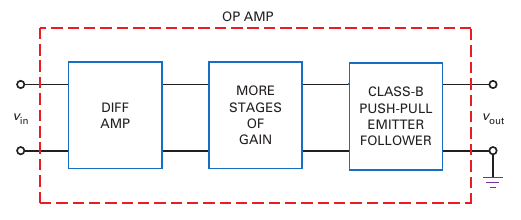
\includegraphics[width=0.8\linewidth]{gambar/fig-16.01}
	\caption{Blok diagram sebuah op amp}
	\label{fig-16.01}
\end{figure}
\end{frame}

\begin{frame}{Pengantar Op Amp}
	\begin{itemize}
		\item Gambar \ref{fig-16.01} adalah diagram blok dari sebuah op amp.
		\item Input stage-nya adalah diff amp, kemudian diikuti dengan lebih banyak tahapan-tahapan penguat dan sebuah Class-B push-pull emitter follower.
		\item Karena diff amp adalah tahapan pertamanya maka hal ini yang menentukan karakteristik input dari op amp.
		\item Sebagian besar op amp adalah single-ended output, seperti pada Gambar \ref{fig-16.01}.
		\item Dengan supply positif dan negatif, single-ended output dirancang untuk memiliki nilai diam nol.
	\end{itemize}
\end{frame}

\begin{frame}{Pengantar Op Amp}
	\begin{itemize}
		\item Tidak semua op amp dirancang seperti Gambar \ref{fig-16.01}.
		\item Beberapa op amp tidak menggunakan Class-B push-pull output, dan ada juga yang memiliki double-ended output.
		\item Op amp juga tidak sesederhana seperti pada Gambar \ref{fig-16.01}.
		\item Rancangan internal dari monolithic op amp sangat rumit, menggunakan ribuan transistor sebagai current mirrors, active load, dan inovasi lainnya yang tidak mungkin di dalam rancangan diskret.
		\item Gambar \ref{fig-16.01} hanya menunjukkan 2 fitur penting yang umumnya digunakan di op amp, yaitu differential input dan single-ended output.
	\end{itemize}
\end{frame}

\begin{frame}{Pengantar Op Amp}
	\begin{figure}
		\centering
		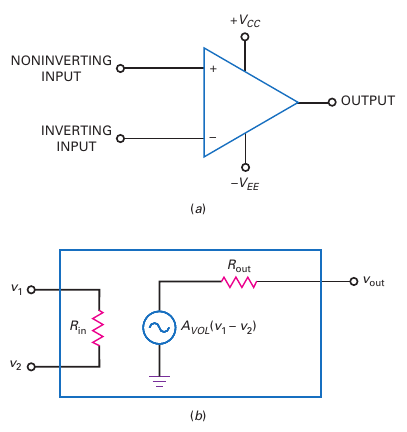
\includegraphics[width=0.4\linewidth]{gambar/fig-16.02}
		\caption{(a) Simbol dari op amp dan (b) rangkaian ekivalen dari op amp}
		\label{fig-16.02}
	\end{figure}
\end{frame}

\begin{frame}{Pengantar Op Amp}
	\begin{itemize}
		\item Gambar \ref{fig-16.02}a adalah simbol skematik dari sebuah op amp.
		\item Memiliki noninverting dan inverting input dan single-ended output.
		\item Idealnya, simbol ini menunjukkan amplifier memiliki voltage gain tak hingga, impedansi input tak hingga, dan nol impedansi input.
		\item Op amp ideal merepresentasikan voltage amplifier yang sempurna dan sering disebut sebagai voltage-controlled voltage source (VCVS).
		\item VCVS ditunjukkan oleh Gambar \ref{fig-16.02}b, dimana $ R_{in} $ bernilai tak hingga dan $ R_{out} $ bernilai nol.
	\end{itemize}
\end{frame}

\begin{frame}{Pengantar Op Amp}
	\begin{figure}
		\centering
		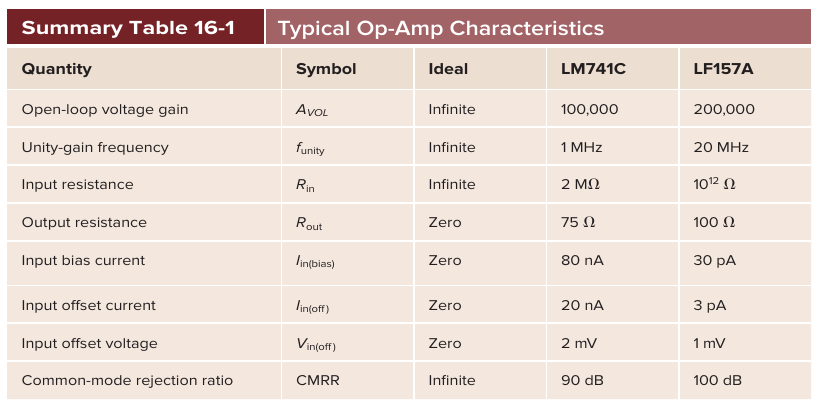
\includegraphics[width=0.8\linewidth]{gambar/tab-16.01}
		\caption{Perbandingan karakteristik op amp ideal dan op amp standar}
		\label{tab-16.01}
	\end{figure}
\end{frame}

\begin{frame}{Pengantar Op Amp}
	\begin{itemize}
		\item Tabel yang ditunjukkan oleh Gambar \ref{tab-16.01} adalah ringkasan dari karakteristik op amp ideal.
		\item Memiliki voltage gain, unity-gain frekuensi, input impedansi, dan CMRR yang bernilai tak hingga.
		\item Memiliki resistor ouput, arus bias, offset yang bernilai nol.
		\item Seperti itulah seharusnya manufaktur membuat op amp, jika mereka mampu.
		\item Namun kenyataannya mereka hanya mampu membuat yang mendekati nilai idealnya saja.
	\end{itemize}
\end{frame}

\begin{frame}{Pengantar Op Amp}
	\begin{itemize}
		\item LM741C memiliki voltage gain sebesar 100000, unity-gain frekuensi sebesar 1 MHz, dan impedansi input sebesar 2 M$ \Omega $, dan seterusnya.
		\item Karena voltage gain yang sangat besar, input offset dapat dengan mudahnya memenuhi op amp.
		\item Sehingga diperlukan komponen eksternal antara input dan output op amp untuk menstabilkan voltage gain.
		\item Contohnya, menggunakan negative feedback untuk menyesuaikan voltage gain keseluruhan menjadi ke nilai yang lebih kecil sebagai ganti operasi linier yang stabil.
	\end{itemize}
\end{frame}

\begin{frame}{Pengantar Op Amp}
	\begin{itemize}
		\item Ketika tidak ada jalur feedback yang digunakan, voltage gain bernilai maksimum yang disebut sebagai open-loop voltage gain, $ A_{VOL} $
		\item Pada Gambar \ref{tab-16.01}, $ A_{VOL} $ dari LM741C bernilai 100000.
		\item Meskipun bukan bernilai tak hingga, open-loop voltage gain ini sangat tinggi.
		\item Contohnya, sebuah input sekecil 10 $ \mu $V akan menghasilkan output sebesar 1 V.
		\item Karena open-loop voltage gain sangat besar, kita dapat menggunakan heavy negative feedback untuk meningkatkan performa keseluruhan rangkaian.
	\end{itemize}
\end{frame}

\begin{frame}{Pengantar Op Amp}
	\begin{itemize}
		\item 741C memiliki unity-gain frequency sebesar 1 MHz, artinya kita memperolah voltage gain hingga 1 MHz.
		\item 741C memiliki input resistance sebesar 2 M$ \Omega $, output resistance sebesar 75 $\Omega$, arus bias input sebesar 80 nA, arus offset input sebsar 20 nA, tegangan offset input sebesar 2 mV, dan CMRR sebesar 90 dB.
		\item Saat resistor yang lebih tinggi dibutuhkan, seorang designer dapat menggunakan op amp BIFET.
		\item JFET digunakan di input stage untuk mendapatkan input bias dan arus offset yang lebih kecil.
		\item Bipolar transistor digunakan pada stage selanjutnya untuk mendapatkan lebih banyak voltage gain.
	\end{itemize}
\end{frame}

\begin{frame}{Pengantar Op Amp}
	\begin{itemize}
		\item LF571A adalah contoh dari op amp BIFET.
		\item Seperti yang ditunjukkan oleh Gambar \ref{tab-16.01}, arus bias inputnya hanya 30 pA dan input resistance adalah $ 10^{12} ~\Omega$.
		\item Memiliki voltage gain 200000 dan unity-gain frequency sebesar 20 MHz.
		\item Dengan menggunakan op amp ini kita bisa mendapatkan voltage gain hingga 20 MHz.
	\end{itemize}
\end{frame}
\section{Op Amp 741}
\begin{frame}{Op Amp 741}
	\begin{itemize}
		\item Monolitic amp $ \mu\text{A709} $ tahun 1965 oleh Fairchild Semiconductor
		\item $ \mu\text{A709} $ memiliki kekurangan $ \rightarrow $ dibuatlah $ \mu\text{A741} $
		\item Banyak manufaktur yang membuat $ \mu\text{A741} $:
		\begin{itemize}
			\item ON Semiconductor: MC1741
			\item Texas Instruments: LM741
			\item Analog Devices: AD741.
		\end{itemize}
		\item Istilah umumnya op amp 741
	\end{itemize}
\end{frame}

\subsection{Standar Industri}
\begin{frame}{Standar Industri}
	\begin{itemize}
		\item Beberapa versi: 741, 741A, 741C, 741E, dan 741N
		\item Bergantung pada karakteristiknya (voltage gain, temp. range, noise level, dll)
		\item 741C (C = \textit{Commercial grade}) $ \rightarrow $ sedikit lebih murah dan paling banyak digunakan
		\item $ A_{VOL} = 100000 $, $ z_{in} = 2 \text{ M}\Omega $, $ z_out = 75~\Omega $
	\end{itemize}
\end{frame}

\begin{frame}{Standar Industri}
	\begin{figure}
		\centering
		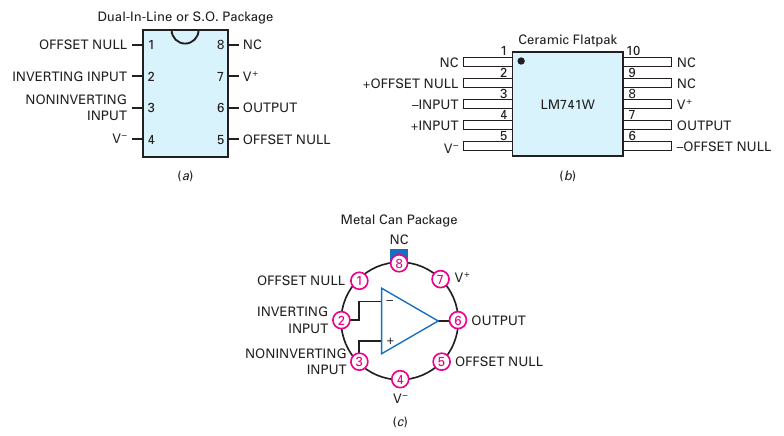
\includegraphics[width=0.7\linewidth]{gambar/fig-16.03}
		\caption{Op amp 741 pinouts (a) dual-in-line, (b) ceramic flatpak, (c) metal can}
		\label{fig-16.03}
	\end{figure}
\end{frame}

\subsection{Rangkaian Ekivalen dari Op Amp 741}
\begin{frame}{Rangkaian Ekivalen dari Op Amp 741}
	\begin{multicols}{2}
		\begin{figure}
			\centering
			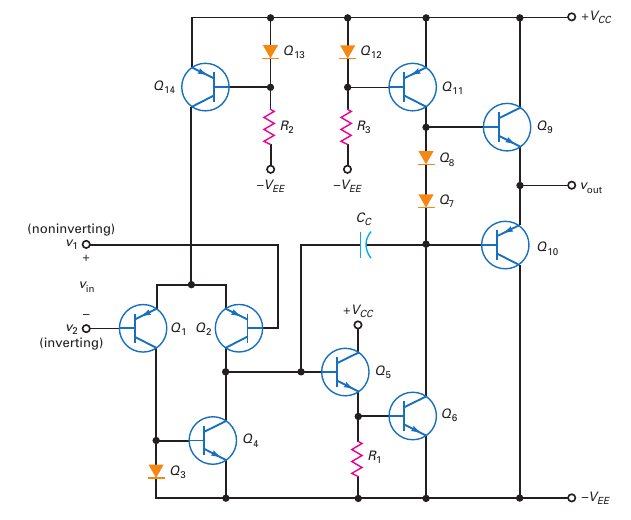
\includegraphics[width=0.9\linewidth]{gambar/fig-16.04}
			\caption{Rangkaian ekivalen dari op amp 741}
			\label{fig-16.04}
		\end{figure}
		\columnbreak
		\begin{itemize}
			\item Input diff amp
			\item Final Stage
			\item Active Loading
			\item Frequency Compensation $ C_{in(M)} = (A_v + 1) C_c $
		\end{itemize}
		\begin{figure}
			\centering
			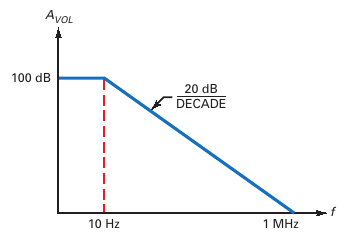
\includegraphics[width=0.5\linewidth]{gambar/fig-16.05}
			\caption{Bode plot $ A_{VOL} $ 741C ideal}
			\label{fig-16.05}
		\end{figure}
	\vfill\null
	\end{multicols}
\end{frame}

\subsection{Bias \& Offset}
\begin{frame}{Bias \& Offset}
	\begin{multicols}{2}
		\begin{figure}
			\centering
			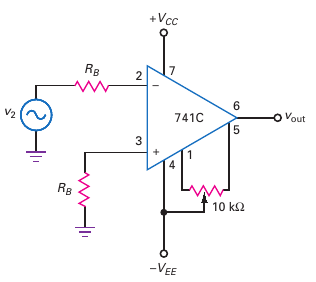
\includegraphics[width=0.8\linewidth]{gambar/fig-16.06}
			\caption{Penggunaan compensation dan nulling 741C}
			\label{fig-16.06}
		\end{figure}
		\columnbreak
		\begin{itemize}
			\item Tidak ada input signal $ \rightarrow $ input bias dan offset $ \rightarrow $ error output
			\item Error output berkurang $ \leftarrow $ base resistor yang sama $ \rightarrow $ hanya menghilangkan arus bias tapi tidak arus offset dan tegangan offset
			\item Solusi: menggunakan rangkaian nulling di datasheet
		\end{itemize}
		\vfill\null
	\end{multicols}
\end{frame}

\subsection{CMRR, MPP, dan $A_{VOL}$}
\begin{frame}{CMRR, MPP, dan $A_{VOL}$}
	\begin{figure}
		\centering
		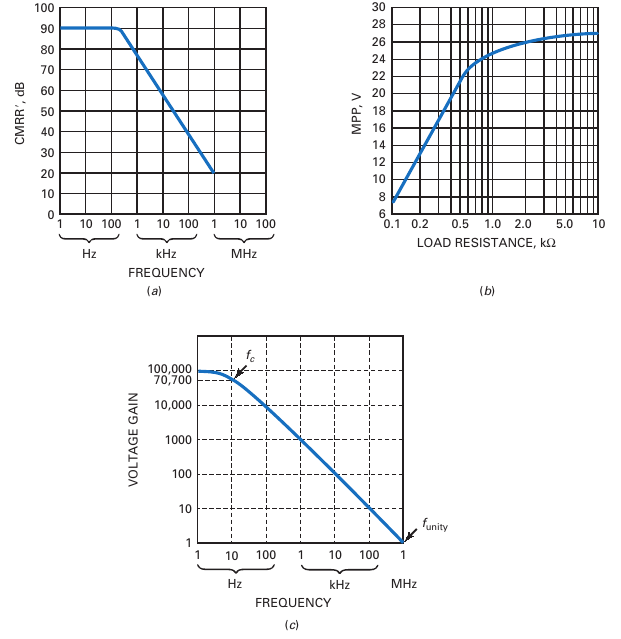
\includegraphics[width=\linewidth]{gambar/fig-16.07}
		\caption{Grafik (a) Common-Mode Rejection Ratio (CMRR), (b) Maximum Peak-to-Peak Output (MPP), dan (c) Open-Loop Voltage Gain $A_{VOL}$ dari 741C}
		\label{fig:fig-07}
	\end{figure}
	\vfill\null
\end{frame}

\subsection{Slew Rate}
\begin{frame}{Slew Rate}
	\begin{multicols}{2}
		\begin{figure}
			\centering
			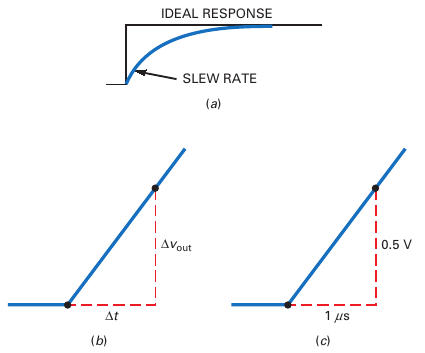
\includegraphics[width=0.8\linewidth]{gambar/fig-16.08}
			\caption{(a) Respon ideal dan aktual terhadap tegangan step input, (b) ilustrasi definisi slew rate, (c) $ S_R = 0.5 \text{ V/}\mu\text{s} $}
			\label{fig:fig-08a}
		\end{figure}
		\columnbreak
		\begin{itemize}
			\item Persamaan slew rate, $ S_R $
			\begin{equation}\label{pers.1}
				S_R = \frac{\Delta v_{out}}{\Delta t}
			\end{equation}
			\item Exponential wave meningkat 0.5 V selama 1 mikrodetik pertama:
			\begin{align*}
				S_R &= \frac{\Delta v_{out}}{\Delta t} \\
				&= \frac{0.5 \text{ V}}{1~\mu\text{s}} \\
				&= 0.5 \text{ V/}\mu\text{s}
			\end{align*}
		\end{itemize}
	\end{multicols}
\end{frame}

\begin{frame}{Slew Rate}
	\begin{figure}
		\centering
		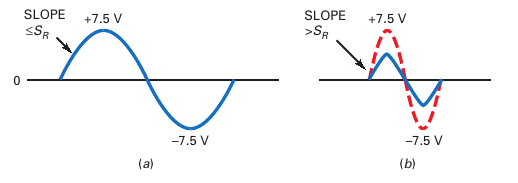
\includegraphics[width=\linewidth]{gambar/fig-16.09}
		\caption{(a) Initial slope dari gelombang sinus, (b) distorsi terjadi jika initial slope melebihi slew rate}
		\label{fig-16.09}
	\end{figure}
\end{frame}

\begin{frame}{Slew Rate}
	\begin{itemize}
		\item Sinyal dan frekuensinya sangat kecil $ \rightarrow $ slew rate bukan masalah
		\item Sinyal dan frekuensinya sangat besar $ \rightarrow $ slew rate akan mendistorsi sinyal ouput
		\[ S_S = 2 \pi f V_p \]
		\item $ S_s $: initial slope dari gelombang sinus, $ f $: frekuensi, $ V_p $: nilai peak
		\begin{align*}
			S_S &\leq S_R \\
			2 \pi f V_p &\leq S_R \\
			f &\leq \frac{S_R}{2 \pi V_p} \\
		\end{align*}
		\begin{equation} \label{pers.16.2}
			f_{max} = \frac{S_R}{2 \pi V_p}
		\end{equation}
	\end{itemize}
\end{frame}

\begin{frame}{Slew Rate}
	\begin{multicols}{2}
		\begin{figure}
			\centering
			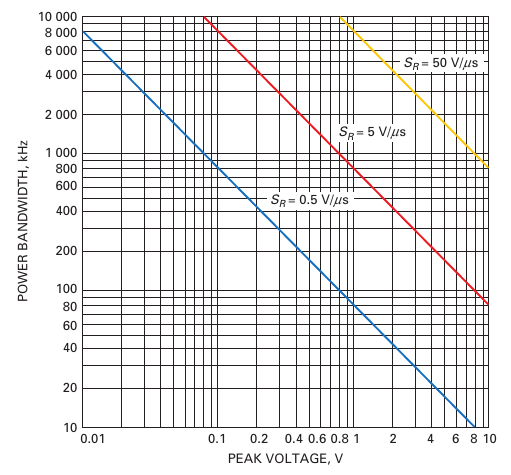
\includegraphics[width=0.8\linewidth]{gambar/fig-16.10}
			\caption{Grafik power bandwidth vs. peak voltage}
			\label{fig-16.10}
		\end{figure}
		\columnbreak
		\begin{itemize}
			\item  $ f_{max} $: power bandwidth atau large-signal bandwidth
		\end{itemize}
	\end{multicols}	
\end{frame}
\section{Inverting Amplifier}
\subsection{Pengantar Inverting Amplifier}
\begin{frame}{Pengantar Inverting Amplifier}
	\begin{itemize}
		\item Inverting amplifier: rangkaian op amp paling dasar
		\item Menggunakan negative feedback untuk menstabilkan keseluruhan voltage gain
		\item Keseluruhan voltage gain perlu distabilkan karena $ A_{VOL} $ sangat besar dan tidak stabil
		\item 741C memiliki $ A_{VOL} $ minimum sebesar 20000 dan $ A_{VOL} $ maksimum lebih dari 200000
	\end{itemize}
\end{frame}

\subsection{Inverting Negative Feedback}
\begin{frame}{Inverting Negative Feedback}
	\begin{figure}
		\centering
		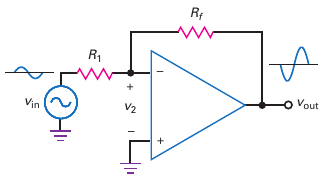
\includegraphics[height=0.5\textheight]{gambar/fig-16.12}
		\caption{Inverting amplifier}
		\label{fig-16.12}
	\end{figure}
\end{frame}

\subsection{Virtual Ground}
\begin{frame}{Virtual Ground}
	\begin{multicols}{2}
		\begin{figure}
			\centering
			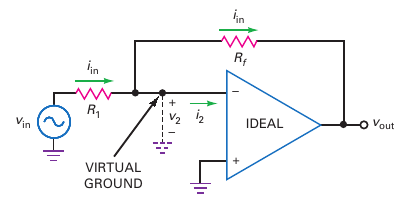
\includegraphics[height=0.4\textheight]{gambar/fig-16.13}
			\caption{Konsep virtual ground}
			\label{fig-16.13}
		\end{figure}
	\columnbreak
		\begin{itemize}
			\item Analisis inverting amplifier lebih mudah
			\item Berdasarkan op amp ideal:
			\begin{itemize}
				\item $ R_{in} = \infty \rightarrow i_2 = 0$
				\item $ A_{VOL} = \infty \rightarrow v_2 = 0 \rightarrow $
			\end{itemize}
			\item Karena $ i_2 = 0 $ maka $ i_{R_f} = i_{in} $
		\end{itemize}
	\end{multicols}
\end{frame}

\subsection{Voltage Gain \& Impedansi Input}
\begin{frame}{Voltage Gain \& Impedansi Input}
	\begin{multicols}{2}
		\begin{figure}
			\centering
			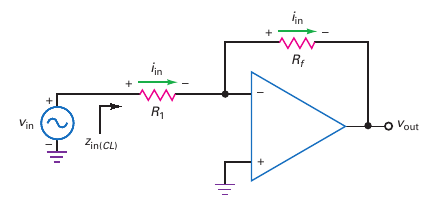
\includegraphics[height=0.4\textheight]{gambar/fig-16.14}
			\caption{Inverting amplifier memiliki arus yang sama yang melewati kedua resistor}
			\label{fig-16.14}
		\end{figure}
	\columnbreak
		\begin{itemize}
			\item Tegangan input: $ v_{in} = i_{in} R_1 $
			\item Tegangan output: $ v_{out} = -i_{in} R_f $
			\item Penguatan tegangan closed-loop:
			\begin{equation}\label{pers.16.3}
				A_{v(CL)} = \frac{-R_f}{R_1}
			\end{equation}
			%\item $ A_{v(CL)} < A_{VOL} $
			\item Impedansi input:
			\begin{equation}\label{pers.16.4}
				z_{in(CL)} = R_1
			\end{equation}
		\end{itemize}
	\end{multicols}
\end{frame}

\subsection{Bandwidth}
\begin{frame}{Bandwidth}
	\begin{multicols}{2}
		\begin{figure}
			\centering
			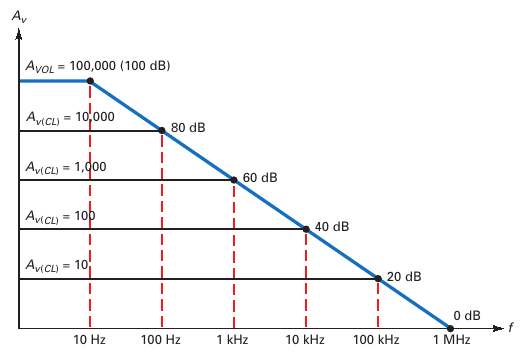
\includegraphics[height=0.6\textheight]{gambar/fig-16.15}
			\caption{Voltage gain yang lebih kecil menghasilkan bandwidth yang lebih besar}
			\label{fig-16.15}
		\end{figure}
	\columnbreak
		\begin{itemize}
			\item 
		\end{itemize}
	\end{multicols}
\end{frame}
\section{Non-inverting Amplifier}

\subsection{Pengantar Non-Inverting Amplifier}
\begin{frame}{Pengantar Non-inverting Amplifier}
	\begin{itemize}
		\item Salah satu rangkaian op amp dasar
		\item Menggunakan negative feedback untuk menstabilkan overall voltage gain
		\item Negative feedback juga meningkatkan impedansi input dan menurunkan impedansi output
	\end{itemize}
\end{frame}

\subsection{Rangkaian Dasar}
\begin{frame}{Rangkaian Dasar}
	\begin{figure}
		\centering
		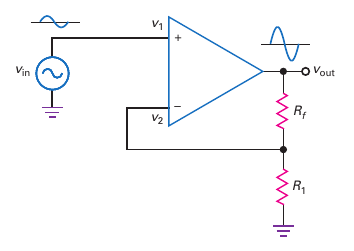
\includegraphics[width=0.5\linewidth]{gambar/fig-16.18}
		\caption{Non-inverting amplifier}
		\label{fig-16.18}
	\end{figure}
\end{frame}

\subsection{Virtual Short}
\begin{frame}{Virtual Short}
	\begin{multicols}{2}
		\begin{figure}
			\centering
			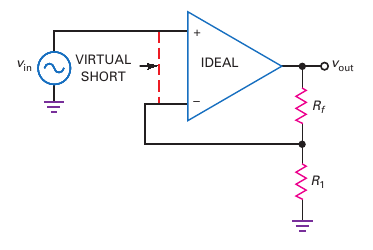
\includegraphics[width=\linewidth]{gambar/fig-16.19}
			\caption{Virtual short}
			\label{fig-16.19}
		\end{figure}
	\columnbreak
		\begin{itemize}
			\item Virtual short digunakan untuk menganalisis noninverting amplifier
			\item Virtual short berdasarkan 2 sifat dari op amp ideal
			\begin{enumerate}
				\item $ R_{in} = \infty \rightarrow i_1 = i_2 = 0$
				\item $ A_{VOL} = \infty \rightarrow v_1 - v_2 = 0$
			\end{enumerate}
		\end{itemize}
	\end{multicols}
\end{frame}

\subsection{Voltage Gain}
\begin{frame}{Voltage Gain}
	\begin{multicols}{2}
		\begin{figure}
			\centering
			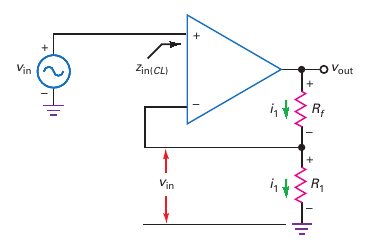
\includegraphics[width=\linewidth]{gambar/fig-16.20}
			\caption{Tegangan input ada di $ R_1 $ dan arus yang sama mengalir di $ R_1 $}
			\label{fig-16.20}
		\end{figure}
		\columnbreak
		\begin{itemize}
			\item Tegangan input: $ v_{in} = i_1 R_1 $
			\item Tegangan output: $ v_{out} = i_1 (R_f + R_1) $
			\item Penguatan tegangan closed-loop:
			\begin{align*}
				A_{v(CL)} = \frac{v_{out}}{v_{in}} = \frac{i_1 (R_f + R_1)}{i_1 R_1} = \frac{R_f + R_1}{R_1}
			\end{align*}
			maka
			\begin{equation}\label{pers.16.12}
				A_{v(CL)} = \frac{R_f}{R_1} + 1
			\end{equation}
		\end{itemize}
	\end{multicols}
\end{frame}

\subsection{Impedansi Input, Bandwidth, Bias \& Offset}
\begin{frame}{Impedansi Input, Bandwidth, Bias \& Offset}
	\begin{itemize}
		\item Karena impedansi input open-loop sudah sangat besar (2 M$ \Omega $ untuk 741C), maka impedansi input closed-loop lebih besar lagi.
		\item Efek negative feedback terhadap bandwidth sama seperti di inverting amplifier
		\[ f_{2(CL)} = \frac{f_{unity}}{A_{v(CL)}} \]
		\item Efek bias dan offset juga sama seperti di inverting amplifier
	\end{itemize}
\end{frame}

\subsection{Error Tegangan Output Mereduksi MPP}
\begin{frame}{Error Tegangan Output Mereduksi MPP}
	\begin{figure}
		\centering
		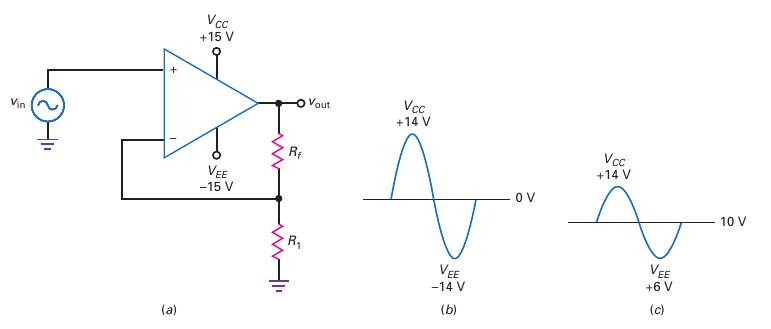
\includegraphics[width=0.9\linewidth]{gambar/fig-16.21}
		\caption{Error tegangan output dapat mereduksi MPP}
		\label{fig-16.21}
	\end{figure}
\end{frame}

\subsection{Contoh Soal 2.10}
\begin{frame}{Contoh Soal 2.10}
	\begin{multicols}{2}
		\begin{center}
			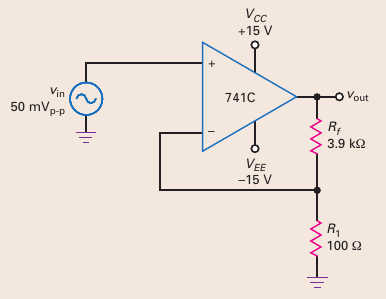
\includegraphics[width=\linewidth]{gambar/fig-16.22a}
		\end{center}
		\columnbreak
		\begin{itemize}
			\item Pertanyaan:
			\begin{itemize}
				\item Berapa penguatan tegangan closed-loop dan bandwidth?
				\item Berapa tegangan output di 250 kHz?
			\end{itemize}
		\end{itemize}
	\end{multicols}
\end{frame}

\begin{frame}{Contoh Soal 2.10}
	\begin{multicols}{2}
		\begin{center}
			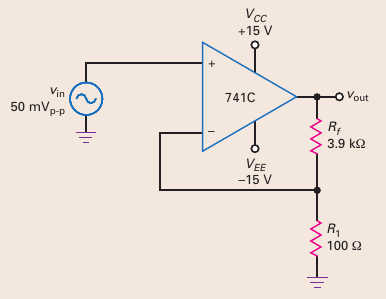
\includegraphics[width=\linewidth]{gambar/fig-16.22a}
		\end{center}
		\columnbreak
		\begin{itemize}
			\item Jawaban:
			\begin{itemize}
				\item Penguatan tegangan closed-loop:
				\begin{align*}
					A_{v(CL)} &= \frac{R_f}{R_1} + 1 = \frac{3.9 \text{ k}\Omega}{100 \text{ k}\Omega} + 1 \\
					&= 40
				\end{align*}
				\item Bandwidth:
				\begin{align*}
					f_{2(CL)}
				\end{align*}
			\end{itemize}
		\end{itemize}
	\end{multicols}
\end{frame}
\section{Aplikasi Op-Amp}

\subsection{Pengantar Aplikasi Op-Amp}
\begin{frame}{Pengantar Aplikasi Op-Amp}
	\begin{itemize}
		\item Aplikasi dari op amp sangat luas sekali dan beraneka ragam
		\item Tidak mungkin menjelaskannya secara komprehensif
		\item Sementara kita fokus pada 2 rangkaian dulu.
	\end{itemize}
\end{frame}

\subsection{The Summing Amplifier}
\begin{frame}{The Summing Amplifier}
	\begin{multicols}{2}
		\begin{figure}
			\centering
			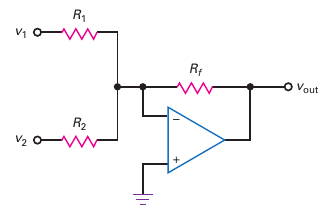
\includegraphics[width=0.9\linewidth]{gambar/fig-16.23a}
			\caption{Rangkaian umming amplifier}
			\label{fig-16.23a}
		\end{figure}
		\begin{itemize}
			\item Menggabungkan 2 atau lebih sinyal analog menjadi satu output
		\end{itemize}
		\columnbreak
		\begin{itemize}
			\item Menguatkan setiap sinyal input
			\item Penguatan setiap channel atau input
			\begin{align*}
				A_{v1(CL)} = \frac{-R_f}{R_1};~~ A_{v2(CL)} = \frac{-R_f}{R_2}
			\end{align*}
			\item Tegangan output
			\begin{equation}\label{pers.16.13}
				v_{out} = A_{v1(CL)}v_1 + A_{v2(CL)} v_2
			\end{equation}
			\item Resistor Thevenin:
			\begin{equation}
				R_{B2} = R_1 \parallel R_2 \parallel R_f \parallel \cdots \parallel R_n
			\end{equation}
		\end{itemize}
	\end{multicols}
\end{frame}

\begin{frame}{The Summing Amplifier}
	\begin{multicols}{2}
		\begin{figure}
			\centering
			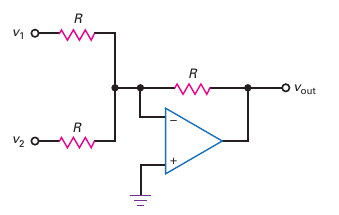
\includegraphics[width=\linewidth]{gambar/fig-16.23b}
			\caption{Rangkaian summing amplifier dengan resistor yang sama}
			\label{fig-16.23b}
		\end{figure}
		\columnbreak
		\begin{itemize}
			\item Tegangan output
			\begin{equation*}
				v_{out} = -(v_1 + v_2 + \cdots + v_n)
			\end{equation*}
		\end{itemize}
	\end{multicols}
\end{frame}

\begin{frame}{The Summing Amplifier}
	\begin{multicols}{2}
		\begin{figure}
			\centering
			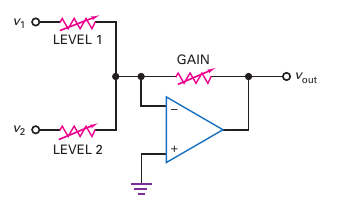
\includegraphics[width=\linewidth]{gambar/fig-16.23c}
			\caption{Rangkaian mixer}
			\label{fig-16.23c}
			\columnbreak
			\begin{itemize}
				\item Menggabungkan sinyal audio
				\item Menurunkan LEVEL 1 $ \rightarrow $ sinyal $ v_1 $ semakin nyaring di output
				\item Menurunkan LEVEL 2 $ \rightarrow $ sinyal $ v_2 $ semakin nyaring di output
				\item Meningkatkan GAIN $ \rightarrow $ kedua sinyal semakin nyaring
			\end{itemize}
		\end{figure}
	\end{multicols}
\end{frame}

\subsection{Voltage Follower}
\begin{frame}{Voltage Follower}
	\begin{multicols}{2}
		\begin{figure}
			\centering
			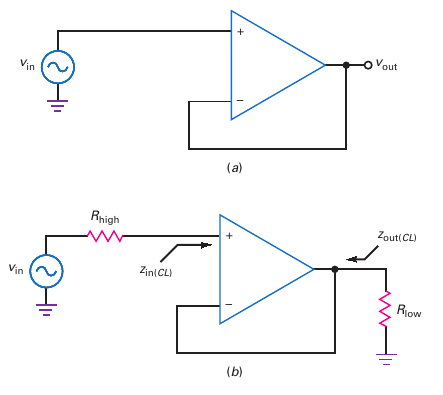
\includegraphics[width=0.9\linewidth]{gambar/fig-16.24}
			\caption{Rangkaian voltage follower}
			\label{fig-16.24}
		\end{figure}
		\columnbreak
		\begin{itemize}
			\item Penguatan tegangan closed-loop:
			\begin{equation}\label{pers.16.15}
				A_{v(CL)} = 1
			\end{equation}
			\item Bandwidth closed-loop:
			\begin{equation}\label{pers.16.16}
				f_{2(CL)} = f_{unity}
			\end{equation}
		\end{itemize}
	\end{multicols}
\end{frame}

\subsection{Contoh Soal 2.12}
\begin{frame}{Contoh Soal 2.12}
	\begin{multicols}{2}
		\begin{center}
			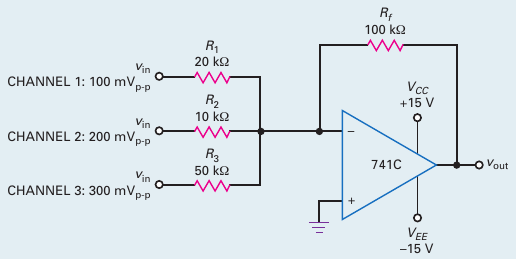
\includegraphics[width=\linewidth]{gambar/fig-16.25}
		\end{center}
		\columnbreak
		\begin{itemize}
			\item Pertanyaan:
			\begin{itemize}
				\item 
			\end{itemize}
		\end{itemize}
	\end{multicols}
\end{frame}
\begin{frame}
	\centering TERIMA KASIH
\end{frame}

\end{document}

